
\begin{frame}
  \frametitle{Ergebnis}
  \begin{block}{Ergebnis}
    \begin{itemize}[<+->]
      \item Anwendbar auf allen \cob
      \item Weitere Robotermodelle werden unterstützt
      \item Einfachere und schnellere Kalibrierung
      \item Sicherheit 
    \end{itemize}
  \end{block}
\end{frame}


\begin{frame}
  \frametitle{Ausblick auf weitere Arbeiten}
  \begin{block} {Weitere Teile einbeziehen}
    \pause
    \begin{itemize}
      \item Laserscanner \pause
      \item Tablett \pause
    \end{itemize}
  \end{block}

  \begin{block} {Genauigkeit erhöhen}
    \pause
    \begin{itemize}
      \item Erweiterung auf ganzen Arbeitsraum \pause
      \item Sampling Strategie verbessern
    \end{itemize}
  \end{block}
\end{frame}

  \bgroup
  \setbeamercolor{background canvas}{bg=black}


\begin{frame}[plain]
\begin{figure}
  \centering
  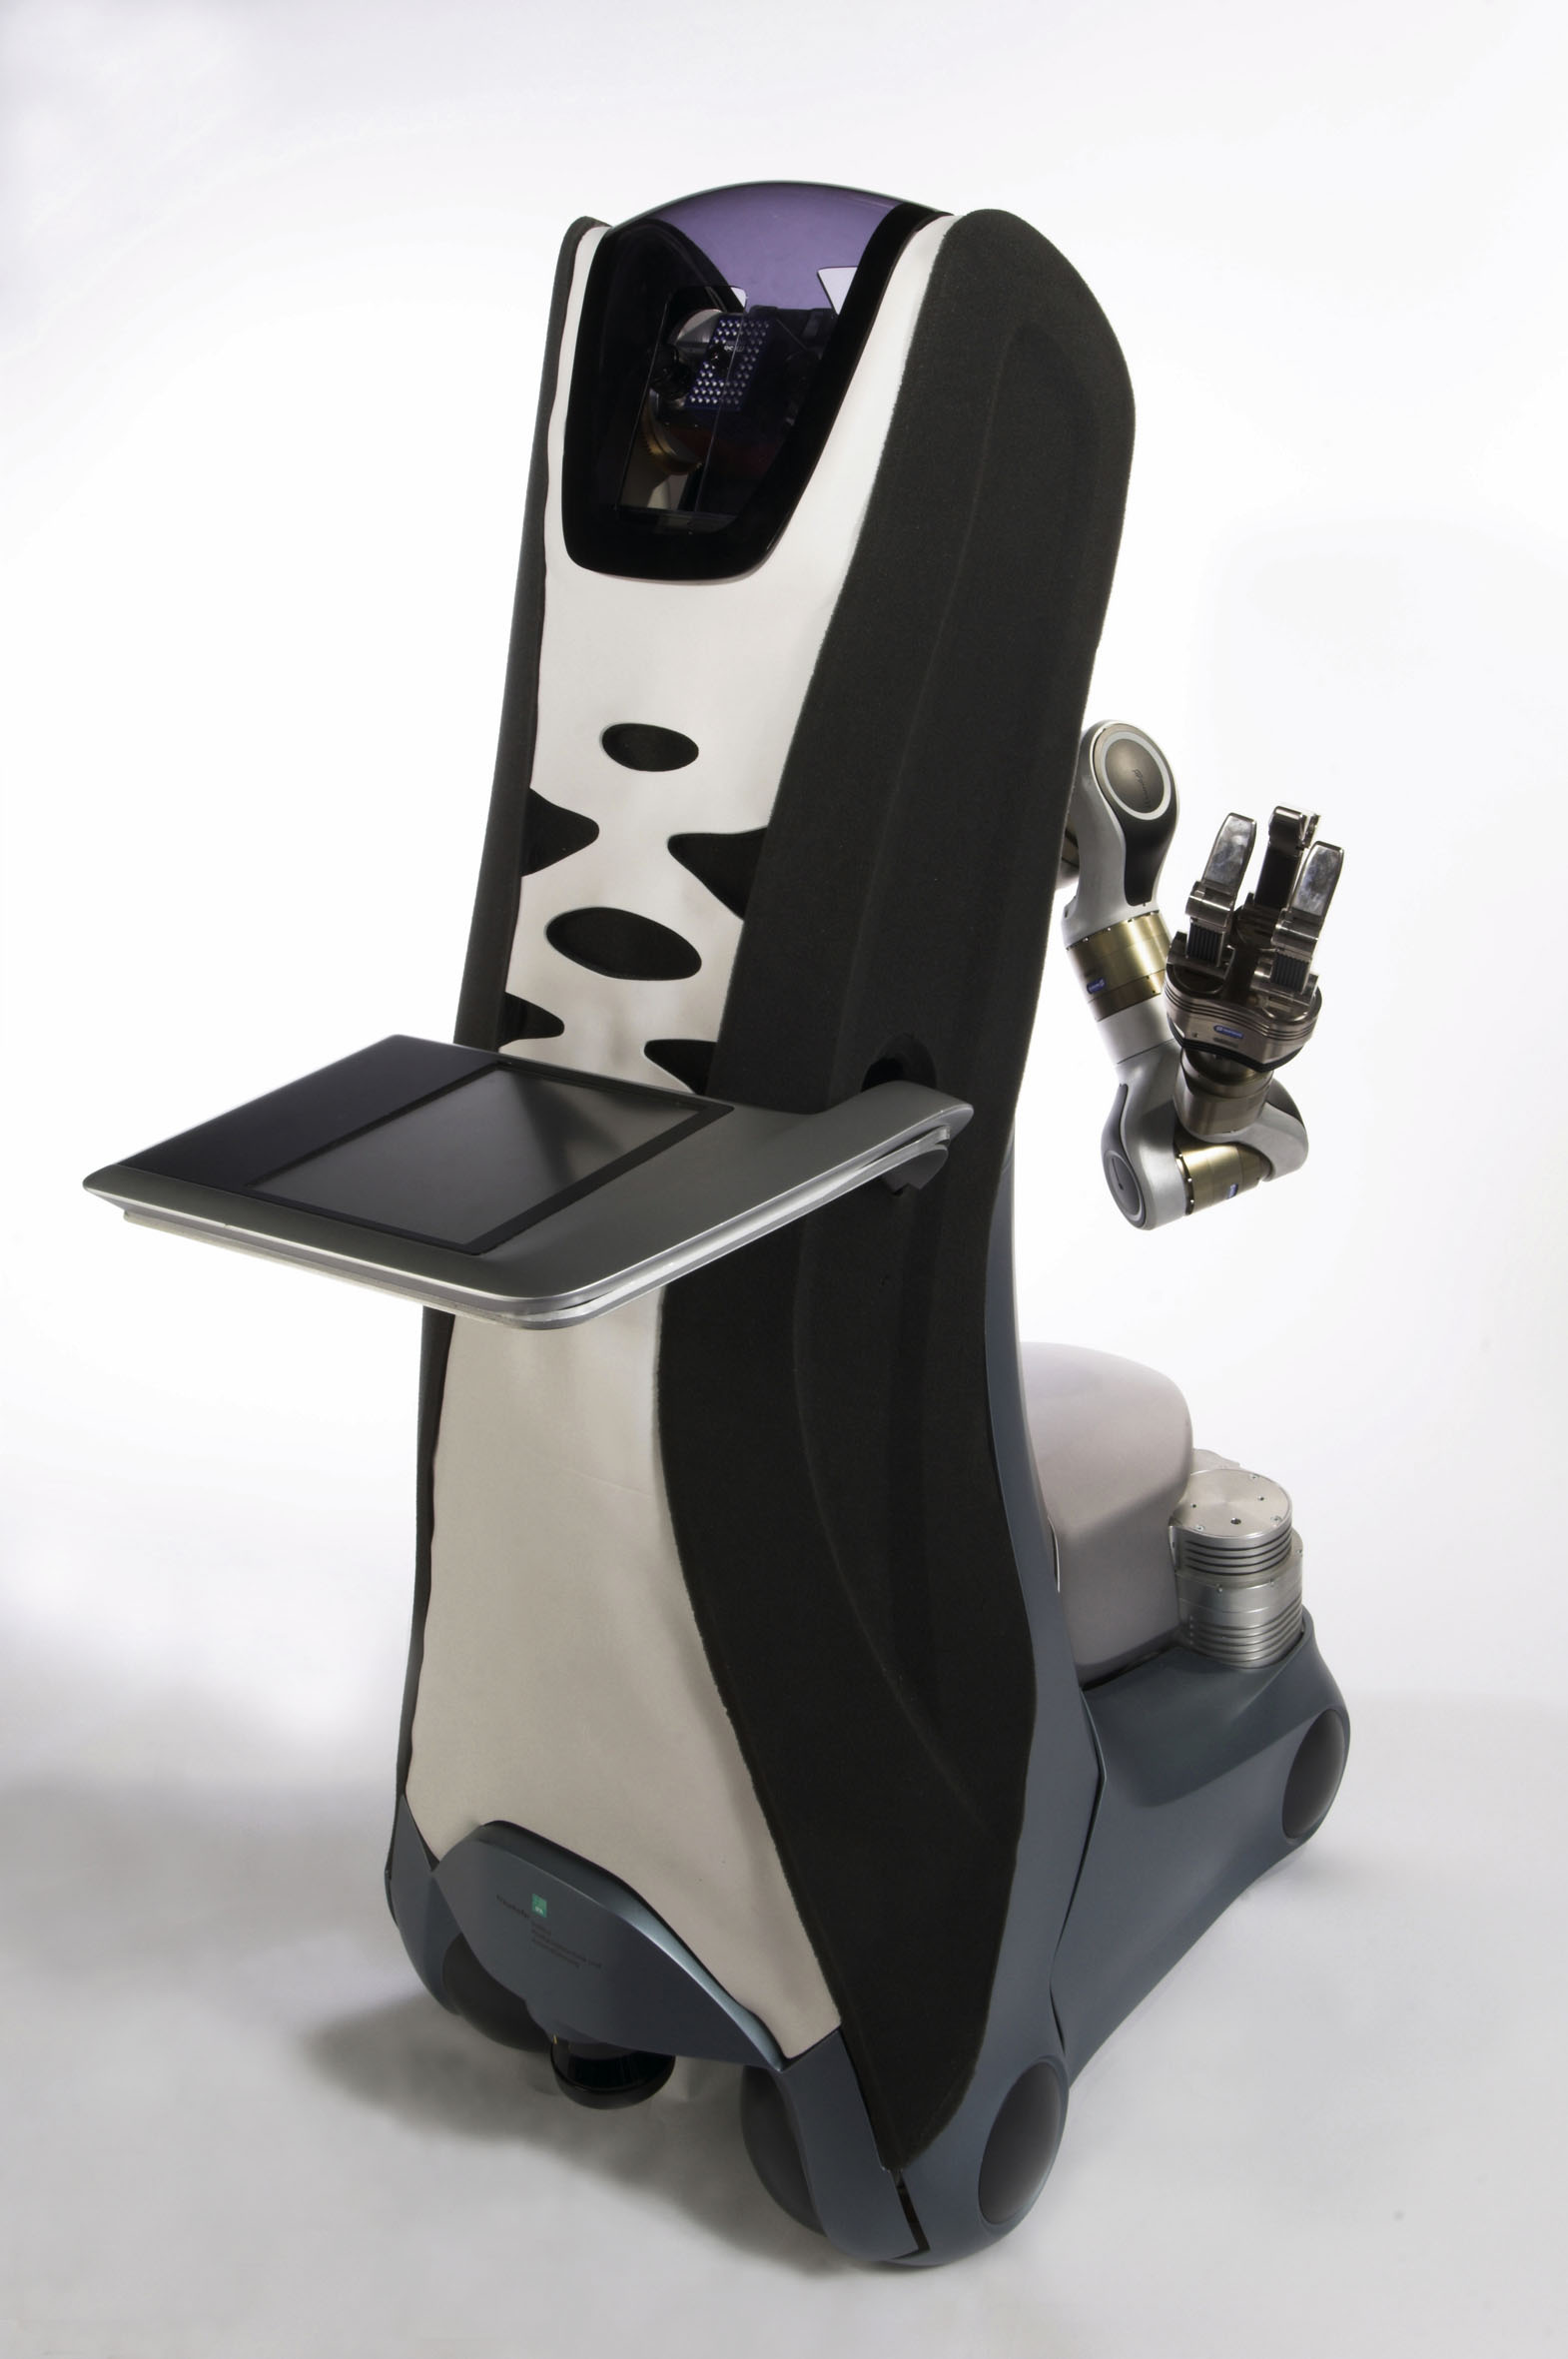
\includegraphics[height=\paperheight]{images/cob}
  \label{fig:cob}
\end{figure}
\end{frame}

\egroup
\begin{frame}
  \frametitle{Abbildungen}
  \begin{description}
    \item[Folie 4] Fraunhofer IPA \url{http://www.care-o-bot.de/Cob3_Download.php}
    \item[Folie 9] Eigene Abbildung
    \item[Folie 20] Fraunhofer IPA: \url{http://www.care-o-bot-research.org/news}
  \end{description}
\end{frame}
